\documentclass[11pt,oneside]{article}
\usepackage[T1]{fontenc}
\usepackage[utf8]{inputenc}
%\DeclareUnicodeCharacter{00A0}{ }
\usepackage[adobe-utopia]{mathdesign}

\usepackage{amsmath}
\usepackage[francais]{babel}
\usepackage[dvips]{graphicx}
%\usepackage{here}
\usepackage{framed}
\usepackage[normalem]{ulem}
\usepackage{fancyhdr}
\usepackage{titlesec}
\usepackage{vmargin}

\usepackage{amsmath}
\usepackage{ifthen}
\usepackage{multirow}
\usepackage{multicol} % Portions de texte en colonnes

%\usepackage{xltxtra} % Logo XeLaTeX
%\usepackage{pst-solides3d}
\usepackage{color}
%\usepackage{colortbl}
\usepackage{titletoc} % Pour la mise en forme de la table des matières

%\usepackage[crop=off]{auto-pst-pdf}
%\usepackage{bclogo}


%\usepackage{longtable}
%\usepackage{flafter}%floatants après la référence
%\usepackage{pst-solides3d}
%\usepackage{pstricks}
%\usepackage{minitoc}
%\setcounter{minitocdepth}{4}
%\usepackage{draftcopy}% "Brouillon"
%\usepackage{floatflt}
%\usepackage{psfrag}
%\usepackage{listings} % Permet d'insérer du code de programmation
%\usepackage{lmodern}
%\usepackage[adobe-utopia,uppercase=upright,greeklowercase=upright]{mathdesign}
%\usepackage{minionpro}
%\usepackage{pifont}
%\usepackage{amssymb}
%\usepackage[francais]{varioref}

\setmarginsrb{1.5cm}{1cm}{1cm}{1.5cm}{1cm}{1cm}{1cm}{1cm}

\definecolor{gris25}{gray}{0.75}
\definecolor{bleu}{RGB}{18,33,98}
\definecolor{bleuf}{RGB}{42,94,171}
\definecolor{bleuc}{RGB}{231,239,247}
\definecolor{rougef}{RGB}{185,18,27}
\definecolor{rougec}{RGB}{255,230,231}
\definecolor{vertf}{RGB}{103,126,82}
\definecolor{vertc}{RGB}{220,255,191}
\definecolor{violetf}{RGB}{112,48,160}
\definecolor{violetc}{RGB}{230,224,236}
\definecolor{jaunec}{RGB}{220,255,191}

\usepackage[%
    pdftitle={SLCI -- Modélisation par transformée de Laplace -- TD},
    pdfauthor={Xavier Pessoles},
    colorlinks=true,
    linkcolor=blue,
    citecolor=magenta]{hyperref}



% \makeatletter \let\ps@plain\ps@empty \makeatother
%% DEBUT DU DOCUMENT
%% =================
\sloppy
\hyphenpenalty 10000

\newcommand{\Pointilles}[1][3]{%
\multido{}{#1}{\makebox[\linewidth]{\dotfill}\\[\parskip]
}}


\begin{document}


\newboolean{prof}
\setboolean{prof}{true}
%------------- En tetes et Pieds de Pages ------------
\pagestyle{fancy}
\renewcommand{\headrulewidth}{0pt}

\fancyhead{}
\fancyhead[L]{%
\noindent\noindent\begin{minipage}[c]{2.6cm}
%Lycée Rouvière PTSI

\includegraphics[width=2cm]{png/logo_ptsi.png}%
\end{minipage}
}

\fancyhead[C]{\rule{12cm}{.5pt}}

\fancyhead[R]{%
\begin{minipage}[c]{3cm}
\begin{flushright}
\footnotesize{\textit{\textsf{Sciences Industrielles\\ de l'Ingénieur}}}%
\end{flushright}
\end{minipage}
}

\renewcommand{\footrulewidth}{0.2pt}

\fancyfoot[C]{\footnotesize{\bfseries \thepage}}
\fancyfoot[L]{\footnotesize{2013 -- 2014} \\ X. \textsc{Pessoles}}
\ifthenelse{\boolean{prof}}{%
\fancyfoot[R]{\footnotesize{CI 2 : SLCI -- Travail Dirigé} \\ \footnotesize{Ch. 2 : Modélisation -- P}}
}{%
\fancyfoot[R]{\footnotesize{CI 2 : SLCI -- Travail Dirigé} \\ \footnotesize{Ch. 2 : Modélisation -- E}}
}


%\begin{center}
%\textit{Centre d'intérêt}
%\end{center}



\begin{center}
 \Large\textsc{CI 2 -- SLCI : Étude du comportement des Systèmes Linéaires Continus Invariants}
\end{center}

\begin{center}
 \large\textsc{Chapitre 2 -- Modélisation des Systèmes Linéaires Continus Invariants}

 \large\textsc{Transformée de Laplace} 
\end{center}

\begin{center}
\textsc{Travail Dirigé} 

\end{center}

%\begin{flushright}
%\textit{D'après ressources de } 
%\end{flushright}
\vspace{.5cm}

\setcounter{subparagraph}{0}

\subsection*{Robot Ericc}

Le robot Ericc est un robot série équipé de 5 axes en série qui lui permettent d'atteindre toutes les positions et toutes les orientations de l'espace. Le dernier axe peut être équipé d'une pince ou d'un outil spécifique. Le robot est par exemple utilisé sur les chaînes de montage dans le domaine de l'automobile afin de souder des éléments de carrosserie de voiture.

%\vspace{.5cm}
\noindent\begin{minipage}[c]{.5\linewidth}
Les axes sont appelés ainsi :
\begin {itemize}
\item axe 1 : axe de lacet;
\item axe 2 : axe d'épaule;
\item axe 3 : axe de coude;
\item axe 4 : axe de poignet;
\item axe 5 : axe de pince. 
\end{itemize}
On s'intéresse uniquement au déplacement de l'axe de lacet. On donne le cahier des charges partiel du robot Ericc. 
\end{minipage} \hfill
\begin{minipage}[c]{.45\linewidth}
\begin{center}
\begin{tabular}{ccc}
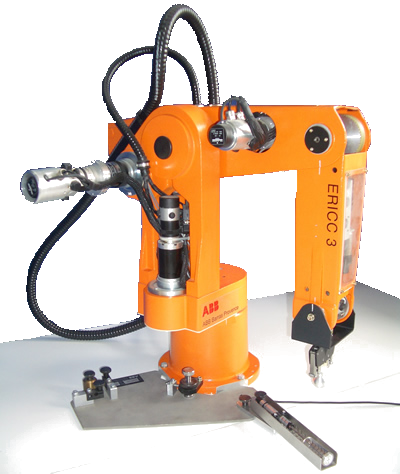
\includegraphics[height=5cm]{png/ericc_1}&&
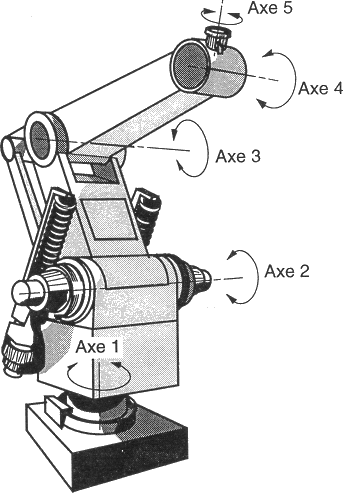
\includegraphics[height=5cm]{png/ericc_2}
\end{tabular}
\end{center}
\end{minipage}


\begin{center}
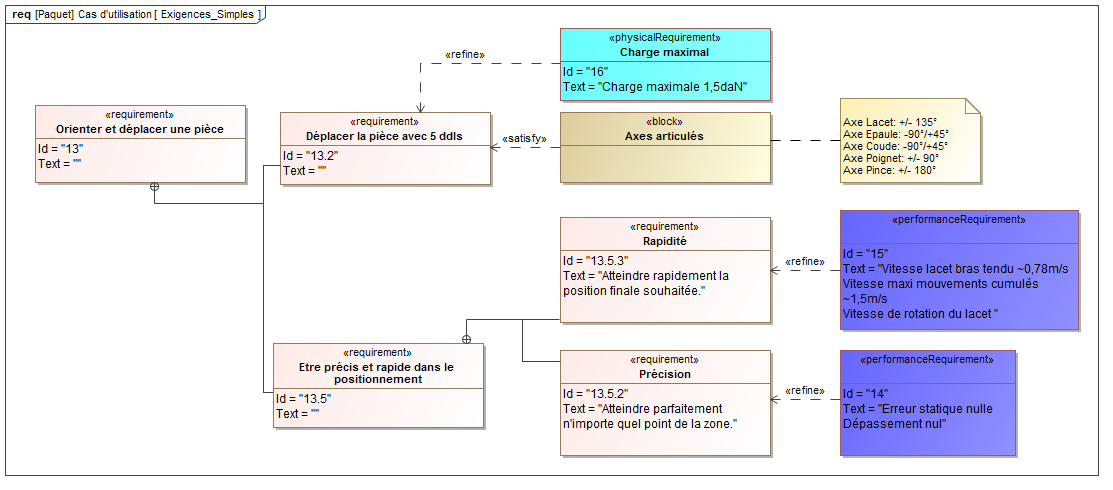
\includegraphics[width=.95\linewidth]{png/req}
\end{center}

\begin{obj}
\begin{minipage}[c]{.5\linewidth}
\textbf{Objectif}

L'objectif est de vérifier les exigences de performance \textit{14}.
\end{minipage}\hfill
\begin{minipage}[c]{.45\linewidth}
\begin{center}
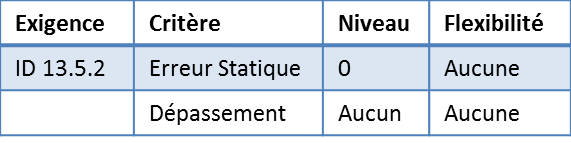
\includegraphics[width=.95\linewidth]{png/cdc}
\end{center}
\end{minipage}
\end{obj}

\noindent\begin{minipage}[c]{.5\linewidth}

Pour déplacer uniquement l'axe de rotation du lacet l'utilisateur peut, par le biais d'un logiciel, piloter l'angle à atteindre par l'axe. Un hacheur permet de distribuer l'énergie électrique dans un motoréducteur. Ce dernier est relié à un système poulie-courroie. La position de l'axe de lacet est mesurée par un codeur incrémental. Le signal du codeur est alors comparé à la consigne de l'utilisateur.

\end{minipage} \hfill
\begin{minipage}[c]{.5\linewidth}
\begin{center}
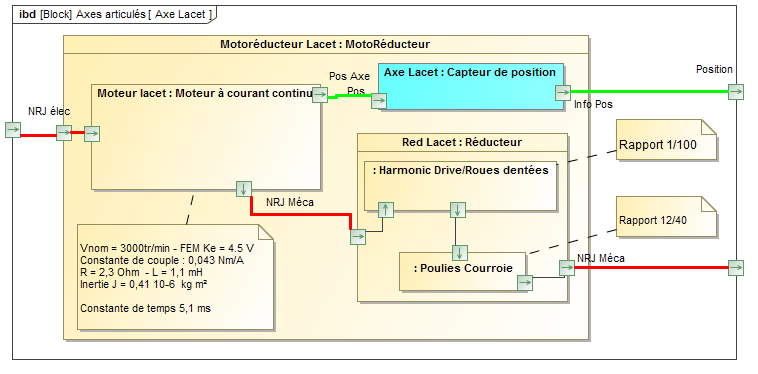
\includegraphics[width=.95\linewidth]{png/bdi_lacet}
\end{center}
\end{minipage}



\subparagraph{}
\textit{Réaliser le schéma-bloc fonctionnel de l'axe de lacet du robot Ericc.}

\ifthenelse{\boolean{prof}}{
\begin{corrige}
\begin{center}
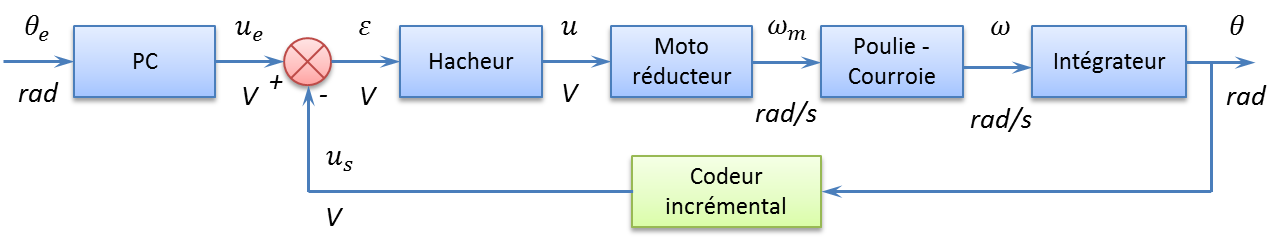
\includegraphics[width=.95\textwidth]{png/schema_bloc}
\end{center}

\textit{Remarque : le réducteur pourrait être sorti du bloc moteur.}
\end{corrige}
}{}

\subsubsection*{Étude de la vitesse du moteur en boucle ouverte}

Un moteur électrique est alimenté par une tension continue. Pour une tension donnée, le moteur tourne à une vitesse donnée. 

Le comportement du moteur est régit par l'équation différentielle suivante : 
$$ 
\omega_m(t) + \tau \dfrac{d\omega_m(t)}{dt} = Ku(t)
$$

en notant :
\begin{itemize}
\item $\omega_m(t)$ la fréquence de rotation du moteur (en $rad/s$);
\item $u(t)$ la tension d'alimentation du moteur (en $V$);
\item $K= 23,26 rad\cdot s^{-1}V^{-1}$ le gain du moteur ;
\item $\tau = 0,51 s$ : constante de temps mécanique du moteur.
\end{itemize}

Le moteur est suivi de deux réducteurs. Le rapport de réduction total est noté $r=\dfrac{12}{4000}$. La fréquence de rotation en sortie des réducteurs $\omega(t)$ peut se calculer ainsi :
$$
\omega(t) = r \omega_m(t)
$$


\subparagraph{}
\textit{On se place dans les conditions de Heaviside. Donner les deux équations dans le domaine de Laplace. Exprimer alors $\Omega(p)$ en fonction de $U(p)$.}

\ifthenelse{\boolean{prof}}{
\begin{corrige}

On a : 
$$
\Omega_m(p) + \tau p\Omega_m(p)= KU(p) \quad  \Omega(p) = r \Omega_m(p)
$$

En conséquence, 
$$
\Omega(p) = \dfrac{rK}{1+\tau p} U(p)
$$
\end{corrige}
}{}

\subparagraph{}
\textit{On sollicite le système par une entrée échelon d'amplitude 1V. Déterminer l'expression de $\Omega(p)$ sous forme littérale.}

\ifthenelse{\boolean{prof}}{
\begin{corrige}
Dans ces conditions, $U(p)=\dfrac{1}{p}$. On a donc :
$$
\Omega(p) = \dfrac{rK}{1+\tau p} \cdot \dfrac{1}{p}
$$
\end{corrige}
}{}

\subparagraph{}
\textit{Après avoir déterminé les valeurs initiales et finales de $\omega(t)$ ainsi que la pente à l'origine, tracer l'allure de $u(t)$ et $\omega(t)$ en indiquant les valeurs numériques.}

\ifthenelse{\boolean{prof}}{
\begin{corrige}
D'après le théorème de la valeur initiale :
$$
\lim \limits_{t\to0} \omega(t) = \lim \limits_{p\to\infty} p\Omega(p) = 0
$$

D'après le théorème de la valeur finale :
$$
\lim \limits_{t\to\infty} \omega(t) = \lim \limits_{p\to0} p\Omega(p) = Kr
$$

La valeur de la pente à l'origine peut être déterminé ainsi : 
$$
\lim \limits_{t\to0} \dfrac{d\omega(t)}{dt} = \lim \limits_{p\to\infty} p^2\Omega(p) = \dfrac{Kr}{\tau}
$$

\end{corrige}
}{}



\subparagraph{}
\textit{Commenter l'allure de la courbe.}

\ifthenelse{\boolean{prof}}{
\begin{corrige}
\end{corrige}
}{}

\subsubsection*{Étude de la position du moteur en boucle ouverte}
On souhaite maintenant avoir accès à la position du moteur en fonction du temps. La position angulaire de l'axe de lacet est notée $\theta$. 

\textit{On se replace dans les conditions où $U(p)$ n'est pas un échelon.}




\subparagraph{}
\textit{Exprimer la relation entre $\theta(t)$ et $\omega(t)$. En déduire la relation entre $\Theta(p)$ et $\Omega(p)$.}

\ifthenelse{\boolean{prof}}{
\begin{corrige}
Le taux de rotation angulaire étant la dérivée de la position angulaire, on a donc :
$$
\dfrac{d\theta(t)}{dt}=\omega(t)
$$

Dans les conditions de Heavside, on a donc :
$$
\Omega(p) = p\Theta(p)
$$

\end{corrige}
}{}



\subparagraph{}
\textit{Exprimer alors $\Theta(p)$ en fonction de $U(p)$.}

\ifthenelse{\boolean{prof}}{
\begin{corrige}
On a : 
$$
\Theta(p) = \dfrac{\Omega(p) }{p} = \dfrac{Kr}{\left(1+\tau p\right)p}U(p)
$$

\end{corrige}
}{}

\subparagraph{}
\textit{On sollicite à nouveau le système par une entrée échelon d'amplitude 1V. Déterminer l'expression de $\Theta(p)$ sous forme littérale.}

\ifthenelse{\boolean{prof}}{
\begin{corrige}
On a : 
$$
\Theta(p) = \dfrac{\Omega(p) }{p} = \dfrac{Kr}{\left(1+\tau p\right)p^2}
$$

\end{corrige}
}{}


\subparagraph{}
\textit{Après avoir déterminé les valeurs initiales et finales de $\theta(t)$ ainsi que la pente à l'origine, tracer l'allure de la courbe en indiquant les valeurs numériques.}

\ifthenelse{\boolean{prof}}{
\begin{corrige}
D'après le théorème de la valeur initiale :
$$
\lim \limits_{t\to0} \theta(t) = \lim \limits_{p\to\infty} p \Theta(p) = \lim \limits_{p\to\infty} p \dfrac{Kr}{\left(1+\tau p\right)p^2} = 0
$$

D'après le théorème de la valeur finale :
$$
\lim \limits_{t\to\infty} \theta(t) = \lim \limits_{p\to0} p \Theta(p)= \lim \limits_{p\to0} p \dfrac{Kr}{\left(1+\tau p\right)p^2} = +\infty
$$

La valeur de la pente à l'origine peut être déterminé ainsi : 
$$
\lim \limits_{t\to0} \dfrac{d\theta(t)}{dt} = \lim \limits_{p\to0} p^2 \Theta(p) = \lim \limits_{p\to\infty} p^2 \dfrac{Kr}{\left(1+\tau p\right)p^2} = Kr
$$

\end{corrige}
}{}


\subparagraph{}
\textit{Commenter l'allure de la courbe. Ce comportement et-il envisageable sur l'axe de lacet du robot ? Commenter. Justifier la nécessité de mettre en \oe{}uvre un asservissement en position.}


\ifthenelse{\boolean{prof}}{
\begin{corrige}
Lorsqu'on alimente un moteur, il tourne. Sa position angulaire augmente donc jusqu'à l'infini. Pour un moteur isolé cela ne pose pas de problèmes. Sur un robot avec des axes en série, la plupart du temps, les axes le peuvent pas tourner indéfiniment (problèmes de câblages ...)

Si on veut avoir un positionnement angulaire du moteur, il est nécessaire d'avoir une boucle de retour afin d'asservir le système.
\end{corrige}
}{}


\subparagraph{}
\textit{Déterminer l'expression de $\Theta(p)$ dans le domaine temporel. On utilisera la transformée de Laplace inverse.}

\ifthenelse{\boolean{prof}}{
\begin{corrige}
$\Theta(p)$ peut se décomposer en élément simple sous la forme suivante :
$$
\Theta(p) 
= \dfrac{Kr}{\left(1+\tau p\right)p^2}
= \dfrac{\alpha}{p} + \dfrac{\beta}{p^2} + \dfrac{\gamma}{1+\tau p}
$$

En multipliant par $p^2$ et en posant $p=0$ on a :
$$
\beta = Kr
$$

En multipliant par $1+\tau p$ et en posant $p=-\dfrac{1}{\tau}$ on a :
$$
\gamma = \dfrac{Kr}{\left(-\dfrac{1}{\tau}\right)^2} = Kr\tau^2
$$

On pose $p=1$ :
$$
\dfrac{Kr}{1+\tau} = \alpha + Kr + \dfrac{Kr\tau^2}{1+\tau} 
\Longleftrightarrow\alpha = \dfrac{1}{1+\tau}\left( Kr - Kr\tau^2 - Kr - Kr\tau\right)
\Longleftrightarrow\alpha = \dfrac{-\tau Kr}{1+\tau}\left(  1 + \tau\right) = -\tau Kr
$$

Au final, 
$$
\Theta(p) 
= \dfrac{-\tau K r}{p} + \dfrac{Kr}{p^2} + \dfrac{Kr\tau^2}{1+\tau p}
= \dfrac{-\tau K r}{p} + \dfrac{Kr}{p^2} + \dfrac{1}{\tau}\cdot \dfrac{Kr\tau^2}{\dfrac{1}{\tau}+ p}
= \dfrac{-\tau K r}{p} + \dfrac{Kr}{p^2} + \dfrac{Kr\tau}{\dfrac{1}{\tau}+ p}
$$

Dans le domaine temporel, on a donc :
$$
\forall t>0 \quad \theta(t) = -\tau K r + Kr t + Kr\tau e^{-\dfrac{t}{\tau}} 
= Kr \left( -\tau +t + \tau e^{-\dfrac{t}{\tau}}\right)
$$
\end{corrige}

\begin{center}
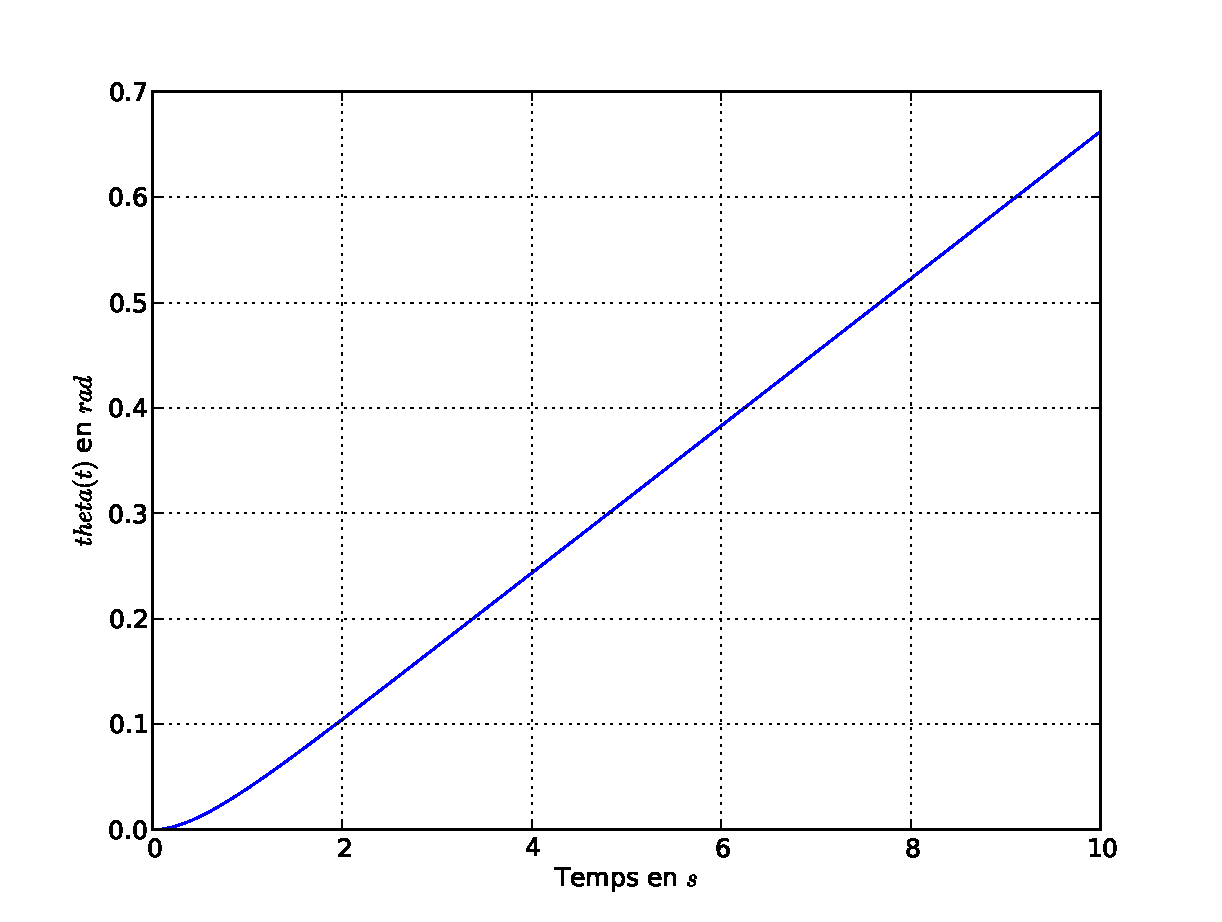
\includegraphics[width=.6\textwidth]{png/figure_1.pdf}
\end{center}

}{}


\subsection*{Étude de l'asservissement en position de l'axe de lacet}
\textit{On se replace dans les conditions où $U(p)$ n'est pas un échelon.}

Afin d'asservir la position angulaire de l'axe de lacet, on utiliser un codeur incrémental. La loi de comportement du codeur est la suivante :
$$
u_s(t)= K_{capt} \cdot \theta(t)
$$

La consigne angulaire donnée par l'utilisateur est adaptée suivant la loi de comportement suivante : 
$$
u_e(t)= K_{Adapt} \cdot \theta_e(t) \quad \text{avec} \quad K_{Adapt} = K_{Capt} = 1 \; V/rad
$$

Un comparateur permet de comparer la tension d'entrée et la tension de sortie : 
$$
\varepsilon(t)=u_e(t) - u_s(t)
$$

Enfin, le hacheur permet d'amplifier la faible tension $\varepsilon(t)$ en tension de commande pour le moteur à courant continu :
$$
u(t)=K_{Ampli} \cdot \varepsilon(t) \quad K_{Ampli}=10
$$

\subparagraph{}
\textit{Justifier que $K_{Adapt} = K_{Capt}$.}

\ifthenelse{\boolean{prof}}{
\begin{corrige}

En reprenant le schéma bloc de la question 1, on se rend compte d'une part que le PC et le capteur réalisent la même opération à savoir convertir une position angulaire en tension. 

De plus, si on se place en régime permanent, dans le cas où l'erreur statique du système serait nulle, on a donc une consigne $\theta_e$ qui est égale à $\theta$. $u_e$ et $u_s$ étant leur image respective, il est donc logique qu'ils soient égaux. En conséquence, l'opération à réaliser par le codeur et par le PC doit être la même ce qui justifie que $K_{Adapt} = K_{Capt}$.

\end{corrige}
}{}


On se place dans les conditions de Heaviside.

\subparagraph{}
\textit{Transformer chacune des 4 équations dans le domaine de Laplace.}

\ifthenelse{\boolean{prof}}{
\begin{corrige}
Dans les conditions de Heaviside, 
\begin{eqnarray*}
U_s(p) = K_{capt} \Theta(p) \\
U_e(p)=K_{Adapt} \Theta_e(p) \\
\varepsilon(p)=U_e(p) - U_s(p) \\
U(p)=K_{Ampli} \cdot \varepsilon(p) 
\end{eqnarray*}
\end{corrige}

}{}


\subparagraph{}
\textit{Exprimer $\Theta(p)$ en fonction de $\Theta_e(p)$.}

\ifthenelse{\boolean{prof}}{
\begin{corrige}
D'après la partie précédente :
$$
\Theta(p)=\dfrac{Kr U(p)}{\left(1+\tau p\right) p}
$$
En conséquence, 
\begin{eqnarray*}
\Theta(p)
&=&\dfrac{Kr}{\left(1+\tau p\right) p} K_{Ampli} \cdot \varepsilon(p) \\
&=&\dfrac{Kr}{\left(1+\tau p\right) p} K_{Ampli} \cdot \left( U_e(p) - U_s(p)\right)\\
&=&\dfrac{Kr}{\left(1+\tau p\right) p} K_{Ampli} \cdot \left( K_{Adapt} \Theta_e(p) - K_{capt} \Theta(p)\right)
\end{eqnarray*}

On a alors :
$$
\Theta(p)\left( 1+  \dfrac{KrK_{Ampli}  K_{capt}}{\left(1+\tau p\right) p} \right)
=\dfrac{KrK_{Ampli} \cdot K_{Adapt}}{\left(1+\tau p\right) p}  \Theta_e(p)
$$

$$
\Longleftrightarrow \Theta(p)\left(  \dfrac{KrK_{Ampli}  K_{capt}+\left(1+\tau p\right) p}{\left(1+\tau p\right) p} \right)
=\dfrac{KrK_{Ampli} \cdot K_{Adapt}}{\left(1+\tau p\right) p}  \Theta_e(p)
$$

Au final :

$$
\Theta(p)
=\dfrac{KrK_{Ampli} \cdot K_{Adapt}}{ KrK_{Ampli}  K_{capt}+\left(1+\tau p\right) p}  \Theta_e(p)
$$
\end{corrige}
}{}

\subparagraph{}
\textit{On désire connaître la réponse indicielle du système (entrée échelon d'amplitude $1\;rad$). Exprimer $\Theta(p)$ en fonction de $\Theta_e(p)$.}

\ifthenelse{\boolean{prof}}{
\begin{corrige}
Pour une réponse indicielle, on a : $\Theta_e(p)=\dfrac{1}{p}$.
En conséquence, 
$$
\Theta(p)
=\dfrac{KrK_{Ampli} \cdot K_{Adapt}}{ KrK_{Ampli}  K_{capt}+\left(1+\tau p\right) p} \cdot\dfrac{1}{p}
$$
\end{corrige}
}{}

\subparagraph{}
\textit{Après avoir déterminé les valeurs initiales et finales de $\theta(t)$ ainsi que la pente à l'origine, tracer l'allure de la courbe en indiquant les valeurs numériques.}

\ifthenelse{\boolean{prof}}{
\begin{corrige}
D'après le théorème de la valeur initiale :
$$
\lim \limits_{t\to0} \theta(t) = \lim \limits_{p\to\infty} p \Theta(p) = 0
$$

D'après le théorème de la valeur finale :
$$
\lim \limits_{t\to\infty} \theta(t) = \lim \limits_{p\to0} p \Theta(p)= 1 
$$

La valeur de la pente à l'origine peut être déterminé ainsi : 
$$
\lim \limits_{t\to0} \dfrac{d\theta(t)}{dt} = \lim \limits_{p\to0} p^2 \Theta(p) = 0
$$
\end{corrige}
}{}

\subparagraph{}
\textit{Déterminer l'expression de $\Theta(p)$ dans le domaine temporel. On utilisera la transformée de Laplace inverse.}

\ifthenelse{\boolean{prof}}{
\begin{corrige}
On a : 
$$
\Theta(p)
=\dfrac{KrK_{Ampli} \cdot K_{Adapt}}{ p\cdot\left( KrK_{Ampli}  K_{capt}  + p +\tau p^2 \right)}  
= \dfrac{\alpha}{p} + \dfrac{\beta+\gamma p}{ KrK_{Ampli}  K_{capt}  + p +\tau p^2 }
$$

En multipliant par $p$ et en posant $p=0$ : 
$$
\alpha = \dfrac{K_{Adapt}}{K_{capt}}  
$$

On multiplie le deux expressions par $p$ et on calcule la limite en $+\infty$ :
D'une part, 
$$
\lim\limits_{p\to+\infty}p \dfrac{KrK_{Ampli} \cdot K_{Adapt}}{ p\cdot\left( KrK_{Ampli}  K_{capt}  + p +\tau p^2 \right)}  
=0
$$

 D'autre part, 
$$
\lim\limits_{p\to+\infty}p \left(\dfrac{\alpha}{p} + \dfrac{\beta+\gamma p}{ KrK_{Ampli}  K_{capt}  + p +\tau p^2 }\right)
= \alpha + \dfrac{\gamma}{\tau}
$$

On a donc : 
$$\gamma = -\alpha\tau = - \dfrac{K_{Adapt}}{K_{capt}}  \tau $$

Enfin, pour $p=1$ on a :
$$
\dfrac{KrK_{Ampli} \cdot K_{Adapt}}{ KrK_{Ampli}  K_{capt}  + 1 +\tau}  
= \dfrac{K_{Adapt}}{    K_{capt}  } + \dfrac{\beta - \dfrac{K_{Adapt}}{K_{capt}}  \tau }{ KrK_{Ampli}  K_{capt}  + 1+\tau  }
$$

$$
\Longleftrightarrow KrK_{Ampli} K_{Adapt} =  \left(KrK_{Ampli}  K_{capt}  + 1 +\tau \right)\dfrac{K_{Adapt}}{K_{capt}}
+\beta - \dfrac{K_{Adapt}}{K_{capt}}  \tau 
$$

$$
\Longleftrightarrow KrK_{Ampli} K_{Adapt} K_{capt}=  \left(KrK_{Ampli}  K_{capt}  + 1 +\tau \right) K_{Adapt}
+\beta K_{capt} - K_{Adapt}  \tau 
$$

$$
\Longleftrightarrow 
\beta  
= \dfrac{-\left(1 +\tau \right) K_{Adapt}  +  K_{Adapt}  \tau }{K_{capt}}
= -\dfrac{K_{Adapt}}{K_{capt}}
$$

Au final : 
On a : 
$$
\Theta(p)
= \dfrac{\dfrac{K_{Adapt}}{K_{capt}}  }{p} + \dfrac{-\dfrac{K_{Adapt}}{K_{capt}}- \dfrac{K_{Adapt}}{K_{capt}}  \tau p}{ KrK_{Ampli}  K_{capt}  + p +\tau p^2 }
= \dfrac{\dfrac{K_{Adapt}}{K_{capt}}  }{p} -\dfrac{K_{Adapt}}{K_{capt}}  \dfrac{1+   \tau p}{ KrK_{Ampli}  K_{capt}  + p +\tau p^2 }
$$

%On a : 
%$$
%F(p)
%=\dfrac{1+   \tau p}{ KrK_{Ampli}  K_{capt}  + p +\tau p^2 } 
%=\dfrac{1}{\tau} \cdot \dfrac{1+   \tau p}{ \dfrac{KrK_{Ampli}  K_{capt}}{\tau}  + \dfrac{p}{\tau} + p^2 } 
%$$
%
%$$
%F(p)
%=\dfrac{1}{\tau} \cdot  \dfrac{1+   \tau p}{\left(p+\dfrac{1}{2\tau} \right)+  \dfrac{KrK_{Ampli}  K_{capt}}{\tau}  -\dfrac{1}{4\tau^2} } 
%$$

Application numérique partielle:

$$
\Theta(p)
= \dfrac{1}{p} -  \dfrac{1+ \tau p}{ KrK_{Ampli}   + p +\tau p^2 }
= \dfrac{1}{p} - \dfrac{\tau}{\tau}\cdot \underbrace{ \dfrac{\dfrac{1}{\tau}+ p}{ \dfrac{KrK_{Ampli}}{\tau}   + \dfrac{1}{\tau}p + p^2 }}_{F(p)}
$$

$$
F(p) = \dfrac{1+ \tau p}{ \left( p + \dfrac{1}{2\tau} \right)-\dfrac{1}{4\tau^2}+\dfrac{KrK_{Ampli}}{\tau}}
$$

On pose $A^2 = -\dfrac{1}{4\tau^2}+\dfrac{KrK_{Ampli}}{\tau}$

On a alors : 
$$
F(p) = \dfrac{\dfrac{1}{\tau}+ p+ \dfrac{1}{2\tau} -  \dfrac{1}{2\tau}}{ \left( p + \dfrac{1}{2\tau} \right)+A^2}
 = \dfrac{ p+ \dfrac{1}{2\tau}}{ \left( p + \dfrac{1}{2\tau} \right)+A^2}+\dfrac{\dfrac{1}{2\tau}}{ \left( p + \dfrac{1}{2\tau} \right)+A^2}
 = \dfrac{ p+ \dfrac{1}{2\tau}}{ \left( p + \dfrac{1}{2\tau} \right)+A^2}+\dfrac{1}{2\tau A}\cdot \dfrac{A}{ \left( p + \dfrac{1}{2\tau} \right)+A^2}
$$


On a donc : 
$$
\forall t>0 \quad \theta(t) =1 - e^{ - \dfrac{t}{2\tau}} \cos\left( At\right)- \dfrac{1}{2\tau A}e^{ - \dfrac{t}{2\tau}}\sin\left( At\right)
$$
\end{corrige}

\begin{center}
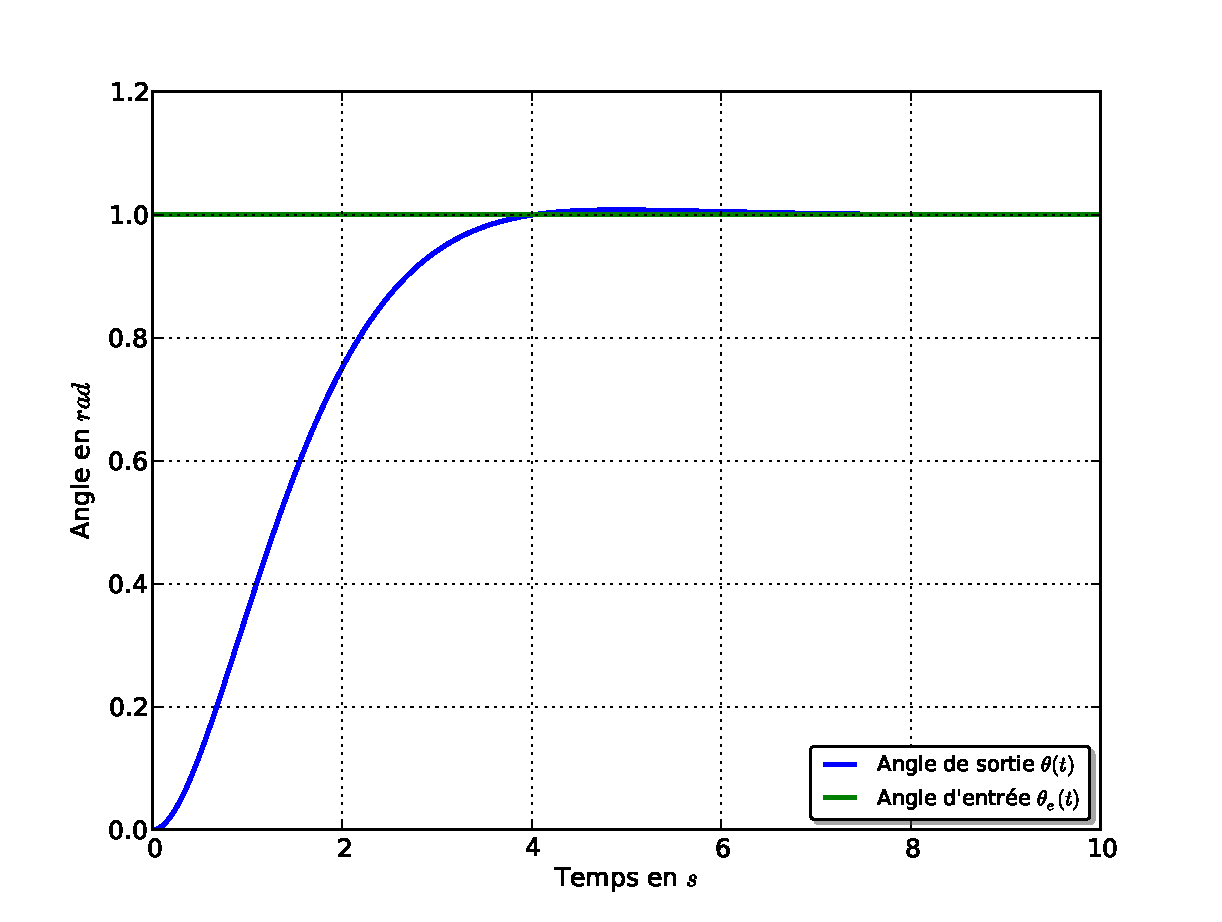
\includegraphics[width=.75\linewidth]{png/figure_2.pdf}
\end{center}
}{}


\subparagraph{}
\textit{Conclure sur la validité du cahier des charges.}

\ifthenelse{\boolean{prof}}{
\begin{corrige}
On observe que le système a un écart statique nul : la consigne était de $1\; rad$ et l'angle atteint par l'axe de lacet est de $1\; rad$. Le critère d'écart statique est donc vérifié. 

En revanche, on observe un léger dépassement de la consigne. En conséquence, le critère de dépassement nul n'est pas vérifié. 
\end{corrige}
}{}
\end{document}
